\subsection{Polymer Architektur}
\label{sec:4_Polymer_Architektur}

Die nachstehende Abbildung \ref{fig:4_polymer_architecture} auf Seite \pageref{fig:4_polymer_architecture} zeigt die Architektur von Polymer.

\begin{figure}[h]
\centering
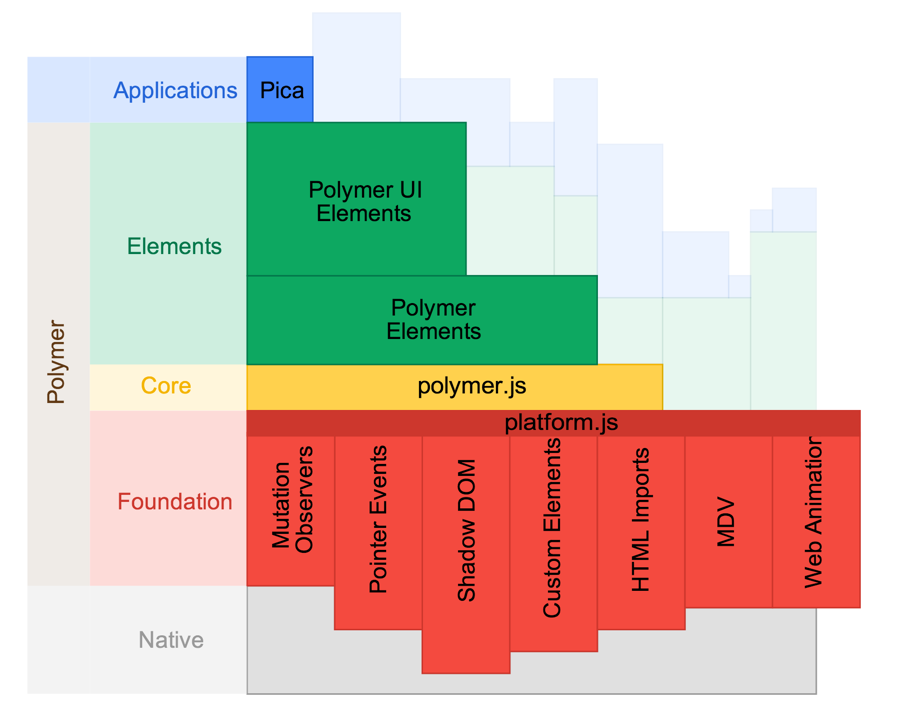
\includegraphics[width=0.8\textwidth,keepaspectratio]{images/polymer_architecture.png}
\caption[
Polymers Architektur, Urldate: 04.2014 \newline
\small\texttt{\url{http://www.polymer-project.org/images/architecture-diagram.svg}}
]{Polymers Architektur}
\label{fig:4_polymer_architecture}
\end{figure}

\begin{description}
\item[Die rote Schicht] visualisiert die Polyfills, die Polymer zur Verfügung stellt. Ein Polyfill ist ein Browser-Fallback, um Funktionen, die in modernen Browsern verfügbar sind, auch in alten Browsern verfügbar zu machen. Diese erlauben die Benutzung von Web-Components. Wichtig hierbei ist, dass die Größe dieser Polyfill-Bibliotheken mit der Weiterentwicklung der Browser abnimmt. Dies bedeutet, dass je mehr Funktionalität von der Spezifikation in den Browsern implementiert ist, desto kleiner sind die Polyfill-Bibliotheken. Der Idealfall für Polymer wäre, dass sämtliche Zusatzbibliotheken, die die nativen Browser-Funktionen emulieren, nicht mehr benötigt werden.
\item[Die gelbe Schicht] stellt die Meinung von Google dar, wie die spezifizierten Browser-Schnittstellen zu Web-Components zusammen verwendet werden sollen. Zusätzlich zu den spezifizierten Technologien werden des Weiteren Funktionalitäten wie \glqq data-bindings\grqq , \glqq change watcher\grqq , \glqq public properties\grqq , etc. bereitgestellt.
\item[Die grüne Schicht] repräsentiert eine umfassende Reihe von Interface-Komponenten. Diese entwickeln sich ständig weiter und basieren auf der gelben, sowie roten Schicht.
\end{description}